\section{Arquitetura do Sistema}
\frame
{
\frametitle{Módulos do Sistema}
Divisão do código em 4 módulos visando o desenvolvimento distribuído:
\begin{itemize}
\item \emph{Core}
\item \emph{GTFS Importer}
\item \emph{Web Service}
\item Cliente
\end{itemize}
}

\frame
{
\frametitle{Visão geral do sistema}
\begin{figure}
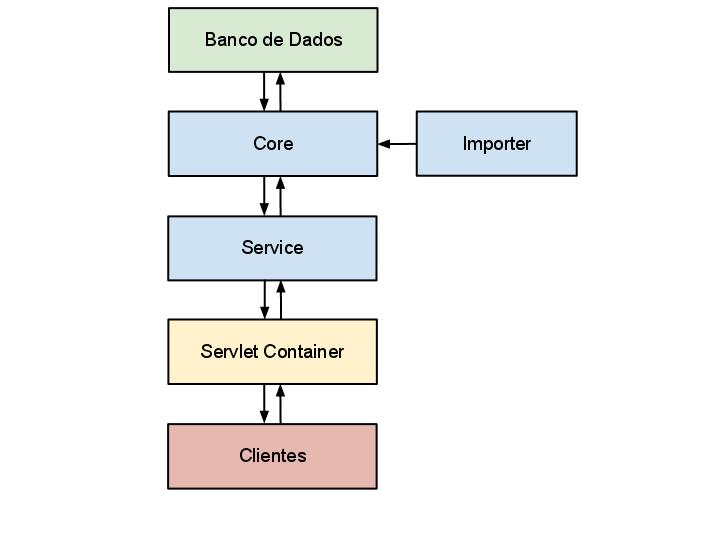
\includegraphics[width=0.7\textwidth]{./imgs/arquitetura.png}
\caption{Representação geral do sistema}
\tiny
Fonte: Autoria própria.
\end{figure}

}

\subsection{Core}
\frame
{
\frametitle{\emph{Core}}
Contém as representações das entidades do sistema:
\begin{itemize}
\item Vértices
\item Relações
\end{itemize}
\begin{figure}
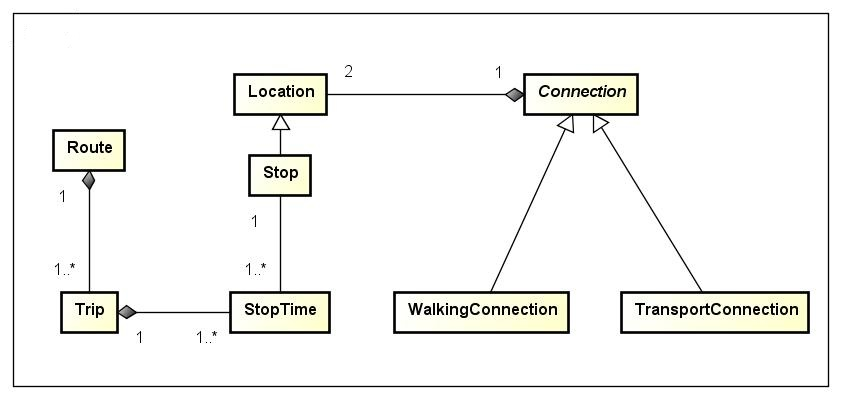
\includegraphics[width=0.8\textwidth]{./imgs/CoreDiagram.png}
\caption{Entidades do \emph{Core}}
\tiny
Fonte: Autoria própria.
\end{figure}

}

\frame
{
\frametitle{\emph{Factories}}
Interface para criação de entidades do \emph{Core}.
\begin{figure}
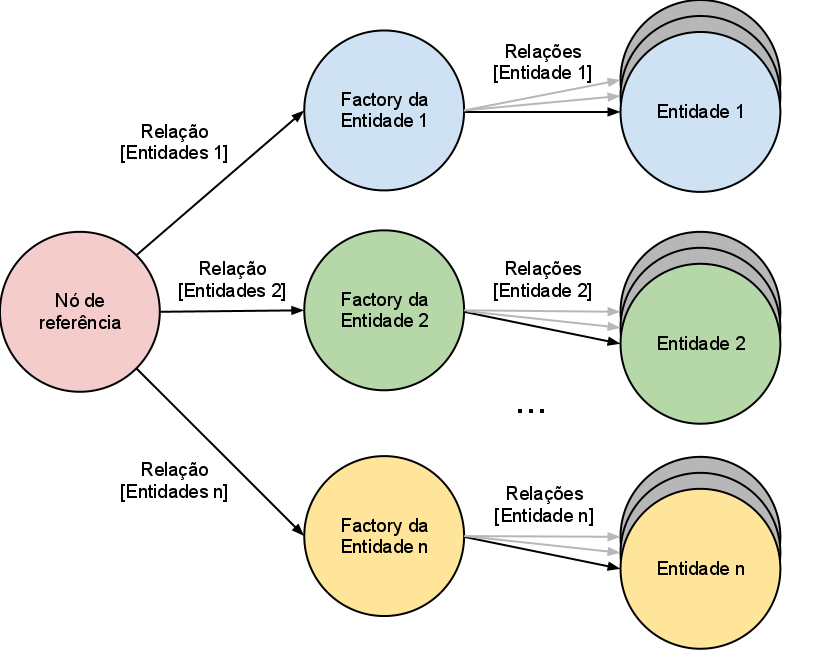
\includegraphics[width=0.6\textwidth]{./imgs/grafoFactory.png}
\caption{Representação de uma entidade no sistema}
\tiny
Fonte: Autoria própria.
\end{figure}
}

\frame
{
\frametitle{\emph{DatabaseController}}
Interface para centralizar o acesso ao banco de dados.
\begin{itemize}
\item Inicia e finaliza transações.
\item Abstração da conexão entre sistema e BD.
\item Referência às \emph{factories}.
\item Algoritmo de busca do caminho mínimo.
\end{itemize}
}

\subsection{Importer}
\frame
{
\frametitle{\emph{GTFS Importer}}
Importação e mapeamento dos arquivos GTFS para o banco de dados.
\begin{itemize}
\item Utiliza métodos do \emph{Core}.
\item Cria relações entre as entidades.
\end{itemize}


\begin{table}
	\tiny
	\caption{Campos obrigatórios a serem importados}
	\begin{tabular}{ll}
		\hline
		\textbf{Arquivo} & \textbf{Campos Obrigatórios} \\
		\hline
		\textbf{Route} & \emph{route ID}: identifica um trajeto \\
				    & \emph{short name}: nome abreviado de um trajeto \\
				    & \emph{long name}: nome completo de um trajeto \\
		\textbf{Trip} & \emph{trip ID}: identifica uma viagem \\ 
				& \emph{route ID} \\ 
				& \emph{service ID}: disponibilidade do serviço por data \\
		\textbf{Stop} & \emph{stop ID}: identifica uma parada ou estação \\
				 & \emph{name}: nome de uma parada ou estação \\
				 & \emph{latitude, longitude}: coordenadas geográficas da parada ou estação \\
		\textbf{StopTime} & \emph{trip ID} \\
				         & \emph{stop ID} \\
				         & \emph{arrival/departure time}: tempo de chegada/partida em uma parada \\
				         & \emph{stop sequence}: ordem das paradas de uma viagem \\
		\hline
	\end{tabular}
	\\ ~ \\
	\tiny
	Fonte: Autoria própria.
\end{table}
}

\frame
{
\frametitle{Algoritmo principal do \emph{Importer}}
\begin{enumerate}
	\item Instanciar \texttt{EntidadeFactory} através da referência à \texttt{DatabaseController}.
	\item Iniciar leitura do arquivo GTFS correspondente à \texttt{Entidade}, sendo que o caminho ao arquivo em questão é fornecido como parâmetro do algoritmo.
	\item Criar nova \texttt{Entidade} através da \texttt{EntidadeFactory} com base nos dados contidos na linha atual do arquivo GTFS.
	\item Adicionar à \texttt{Entidade} criada no passo 3 seus atributos especificados na linha atual.
	\item Se ainda existir linhas não lidas no arquivo GTFS, ler a próxima linha e voltar ao passo 3.
	\item Caso contrário, finalizar a importação.
\end{enumerate}
}

\subsection{Web Service}
\frame
{
\frametitle{\emph{Web Service}}
Servlets responsáveis por executar consultas na base de dados construída através do Importer.

\begin{enumerate}
\item Recebimento dos pontos do Cliente.
\item Criação dos nós de origem e destino no banco de dados.
\item Criação de conexões a pé entre os nós de origem e destino e todas as paradas.
\item Execução da consulta de caminho mínimo no grafo através de \texttt{DatabaseController}.
\item Serialização do resultado da consulta para formato JSON.
\item Envio do resultado ao Cliente.
\end{enumerate}
}

\subsection{Cliente}
\frame
{
\frametitle{Cliente \emph{Web}}
Página \emph{web} em JavaScript (jQuery) que recolhe e envia ao \emph{Web Service} as seguintes informações do usuário (HTTP POST):
\begin{itemize}
\item Pontos de origem/destino (\emph{geocoding}).
\item Horário de partida.
\end{itemize}
Recebe (JSON) e mostra o resultado da busca.
\begin{itemize}
\item No mapa (diferenciando rotas por cor) (Google Maps).
\item Sequência de passos.
\end{itemize}
}

\frame
{
\frametitle{Interface do Cliente \emph{Web}}
\begin{figure}
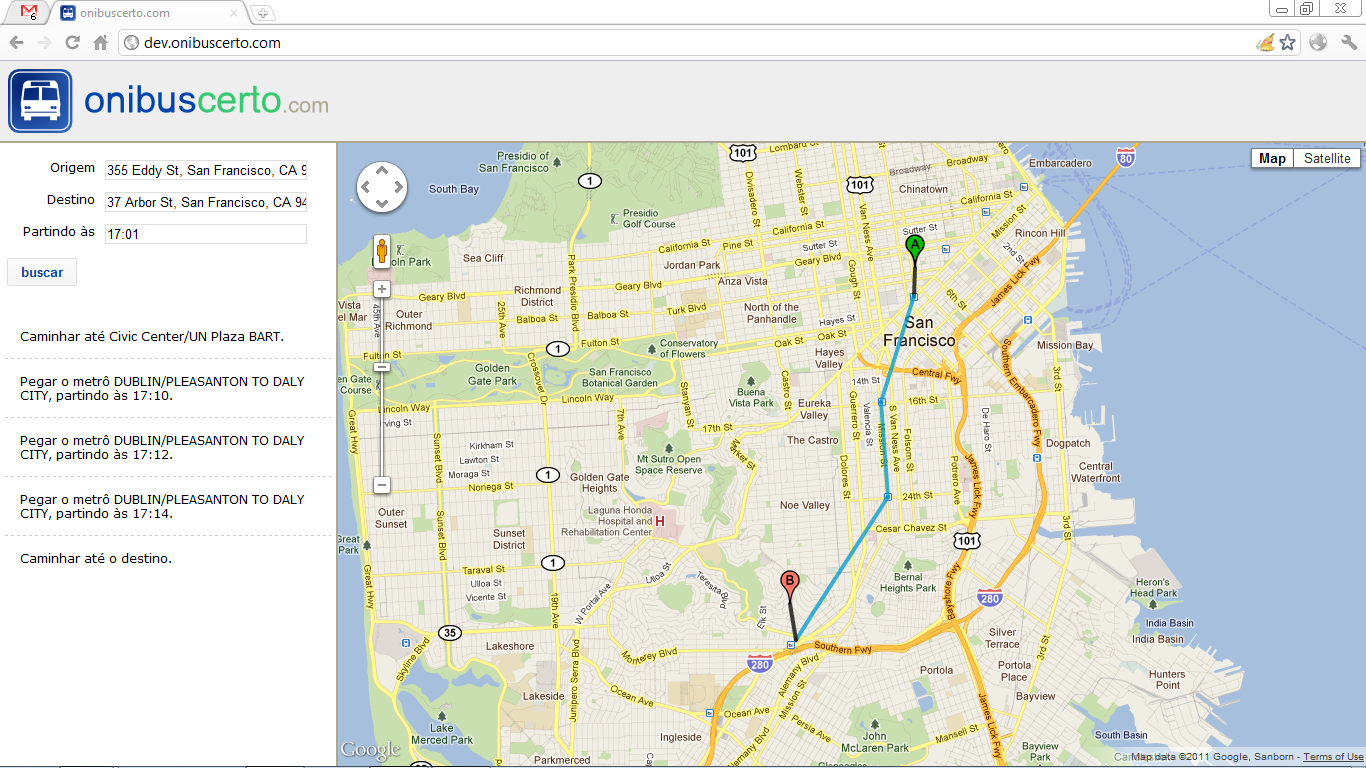
\includegraphics[width=1\textwidth]{./imgs/clienteweb.png}
\caption{Interface do cliente \emph{web}}
\tiny
Fonte: Autoria própria.
\end{figure}
}
